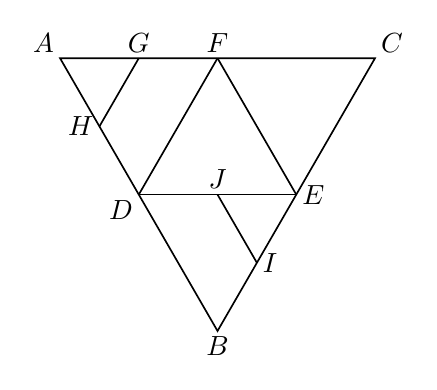
\begin{tikzpicture}[x=1cm,y=1cm,font=\normalsize,
 geometry edge/.style={solid,line width=.6pt},
 geometry mark/.style={solid,line width=.6pt},
 geometry label/.style={font=\normalsize,inner sep=2pt}]
\coordinate (A) at (0,0);
\coordinate (C) at (4,0);
\coordinate (B) at (2.000000,-3.464102);
\coordinate (D) at (1.000000,-1.732051);
\coordinate (E) at (3.000000,-1.732051);
\coordinate (F) at (2.000000,0.000000);
\coordinate (G) at (1.000000,0.000000);
\coordinate (H) at (0.500000,-0.866025);
\coordinate (I) at (2.500000,-2.598076);
\coordinate (J) at (2.000000,-1.732051);
\draw[geometry edge] (A)--(C)--(B)--cycle;
\draw[geometry edge] (D)--(E);
\draw[geometry edge] (D)--(F);
\draw[geometry edge] (F)--(E);
\draw[geometry edge] (G)--(H);
\draw[geometry edge] (I)--(J);
\node[geometry label,above left] at (A) {$A$};
\node[geometry label,above] at (G) {$G$};
\node[geometry label,above] at (F) {$F$};
\node[geometry label,above right] at (C) {$C$};
\node[geometry label,left] at (H) {$H$};
\node[geometry label,below left] at (D) {$D$};
\node[geometry label,above] at (J) {$J$};
\node[geometry label,right] at (E) {$E$};
\node[geometry label,right] at (I) {$I$};
\node[geometry label,below] at (B) {$B$};
\end{tikzpicture}